\documentclass[tikz,border=10pt]{standalone}
\usetikzlibrary{angles,quotes}
\begin{document}
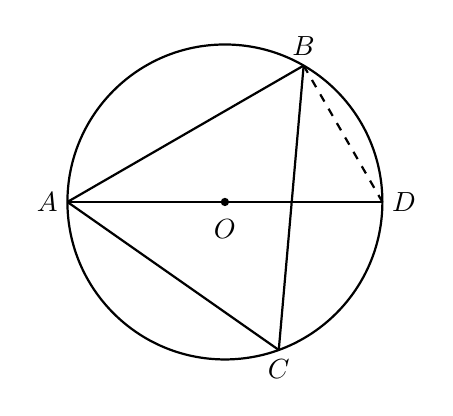
\begin{tikzpicture}    
% 1. 定义圆心和半径    
\coordinate (O) at (0,0);    
\def\r{2} % 半径为 2        
% 2. 绘制圆    
\draw[thick] (O) circle (\r);    
\fill (O) circle (1.5pt) node[below=3pt] {$O$};        
% 3. 定义关键点坐标    
% A 和 D 在直径两端    
\coordinate (A) at (-\r, 0);    
\coordinate (D) at (\r, 0);    
% B 和 C 设定在圆周上 (角度可调节)    
\coordinate (B) at (60:\r);    
\coordinate (C) at (-70:\r);        
% 4. 绘制实线线段    
\draw[thick] (A) -- (D); % 直径    
\draw[thick] (A) -- (B);    
\draw[thick] (B) -- (C);    
\draw[thick] (A) -- (C);        
% 5. 绘制虚线线段    
\draw[thick, dashed] (B) -- (D);        
% 6. 标注点符号    
\node[left]  at (A) {$A$};    
\node[above] at (B) {$B$};    
\node[below] at (C) {$C$};    
\node[right] at (D) {$D$};    
\end{tikzpicture}
\end{document}